\documentclass{article}
\usepackage[margin=1in]{geometry}
\usepackage[T1]{fontenc}
\usepackage{csquotes}
\usepackage{url}
\usepackage{graphicx}
\usepackage{caption}
\usepackage{xcolor,colortbl}
\usepackage{textcomp} 
\usepackage{listings}
\usepackage{enumitem}
\usepackage{float}
\usepackage{subfig}
\usepackage{hyperref}
\usepackage{indentfirst}
\renewcommand{\familydefault}{\sfdefault}

\newcommand{\mc}[2]{\multicolumn{#1}{c}{#2}}
\definecolor{Gray}{gray}{0.95}
\definecolor{LightCyan}{rgb}{0.88,1,1}

\newcolumntype{a}{>{\columncolor{Gray}}l}
\newcolumntype{b}{>{\columncolor{white}}c}

\graphicspath{{./img/}}


% Listings

\lstset{numbers=none,numberblanklines=false,columns=fullflexible,basicstyle=\ttfamily,linewidth=\columnwidth,breaklines=true}

\newcommand{\CodeSymbol}[1]{\bfseries\textcolor{violet}{#1}}   % Code associated to defining styles
\newcommand{\InitColor}[1]{\bfseries\textcolor{orange}{#1}}   % Code associated to defining styles
\newcommand{\RedColor}[1]{\bfseries\textcolor{red}{#1}}   % Code associated to defining styles
\newcommand{\PairColor}[1]{\bfseries\textcolor{blue}{#1}}   % Code associated to defining styles
\newcommand{\CustomFunction}[1]{\bfseries\textcolor{magenta}{#1}}   % Code associated to defining styles

\definecolor{codegray}{gray}{0.95}
\definecolor{commentgray}{gray}{0.35}

\makeatletter

\lstdefinelanguage{clingo}{%
  basicstyle=\footnotesize\ttfamily,%
  backgroundcolor=\color{codegray},%
  showstringspaces=false,%
  alsoletter=0123456789,%
  columns=fullflexible,%
  resetmargins=true,%
  breaklines=true,%
  keywords=[3]{&,&dom,&sum,&diff,&show},%
  morecomment=[l]{\#\ },%
  morecomment=[l]{\%\ },%
  morestring=[b]",%
  stringstyle={\itshape},%
  commentstyle={\color{commentgray}},%
  literate={init}{{\InitColor{init}}}1
           {not}{{\RedColor{not }}}1
           {pair}{{\PairColor{pair}}}1
           {onNode}{{\CustomFunction{onNode}}}1
           {occurs}{{\CustomFunction{occurs}}}1
           {action}{{\CustomFunction{action}}}1
           {move}{{\CodeSymbol{move}}}1
           {robot}{{\CodeSymbol{robot}}}1
           {robotMove}{{\CustomFunction{robotMove}}}1
           {onRobot}{{\CustomFunction{onRobot}}}1
           {deliver}{{\CustomFunction{deliver}}}1
           {onShelf}{{\CustomFunction{onShelf}}}1
           {order}{{\CustomFunction{order}}}1
           {goal}{{\CustomFunction{goal}}}1
           {pickingStation}{{\CustomFunction{pickingStation}}}1
           {nodeAt}{{\CodeSymbol{nodeAt}}}1
           {object}{{\CodeSymbol{object}}}1
           {value}{{\CodeSymbol{value}}}1
           {\#const}{{\CodeSymbol{\#const }}}1
           {\#show}{{\CodeSymbol{\#show }}}1
           {\#minimize}{{\CodeSymbol{\#minimize }}}1
           {\#base}{{\CodeSymbol{\#base }}}1
           {\#theory}{{\CodeSymbol{\#theory }}}1
           {\#count}{{\CodeSymbol{\#count }}}1
           {\#external}{{\CodeSymbol{\#external }}}1
           {\#program}{{\CodeSymbol{\#program }}}1
           {\#script}{{\CodeSymbol{\#script }}}1
           {\#end}{{\CodeSymbol{\#end }}}1
           {\#heuristic}{{\CodeSymbol{\#heuristic }}}1
           {\#edge}{{\CodeSymbol{\#edge }}}1
           {\#project}{{\CodeSymbol{\#project }}}1
           {\#show}{{\CodeSymbol{\#show }}}1
           {\#sum}{{\CodeSymbol{\#sum }}}1%
}

\newcommand\opstyle{\CodeSymbol} % <--- customise operator style here

% Hook into listings
\lst@AddToHook{OutputOther}{\ProcessOther@silmeth}

% helper macro
\newcommand\ProcessOther@silmeth
{%
  \ifnum\lst@mode=\lst@Pmode%     % If we're in `Processing' mode...
    \def\lst@thestyle{\opstyle}%  % ... redefine the style locally
  \fi%
}

\makeatother

\newcommand{\Sim}{{\raise.17ex\hbox{\ensuremath{\scriptstyle\sim}}}}

\begin{document}

\title{SER 222: ADJ Problem 1}
\author{Claudio Rodriguez Rodriguez}
\maketitle

% task_struct - from <linux/sched.h> <-- defined here

% for_each_process - from <linux/sched/signal.h> <-- defined here (MACRO)

% list_for_each - from #include <linux/list.h> <-- defined here (MACRO)
% list_entry - from #include <linux/list.h>  <-- defined here (MACRO)
% list_head - from #include <linux/list.h>

% module_param - from #include <linux/moduleparam.h> <-- defined here (MACRO)
% MODULE_PARM_DESC - from #include <linux/moduleparam.h> <-- defined here (MACRO)

% printk - from <linux/kernel.h> 
% defined in #include <linux/printk.h>
% function

% print_header
% print_row
% init_rodriguez_rodriguez_lkm_module
% exit_rodriguez_rodriguez_lkm_module

\section{Analysis for YouTube Thumbnail Generator}

\subsection{Thumbnails}


\begin{figure}[h!]
\centering
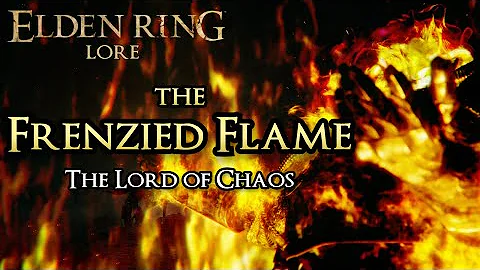
\includegraphics[width=0.5\textwidth]{Arlum Grim.png}
\caption{The Frenzied Flame Lore | Three Fingers of Chaos | Elden Ring by Arlum Grim}
\label{fig:thumbnail1}
\end{figure}

\begin{figure}[h!]
  \centering
  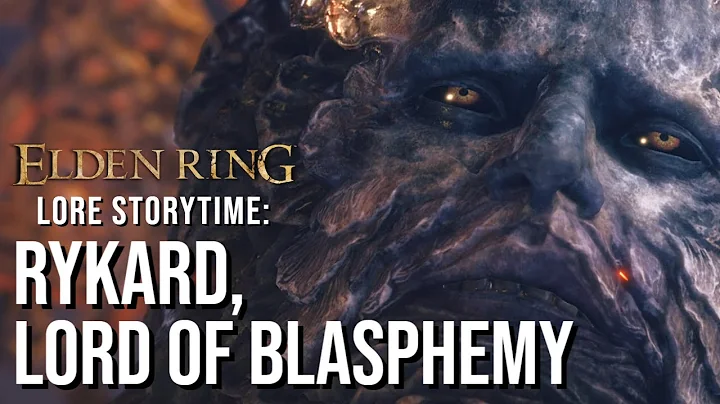
\includegraphics[width=0.5\textwidth]{KiteTales and Flex.png}
  \caption{Elden Ring Lore Storytime: Rykard, Lord of Blasphemy by KiteTales \& Flex}
  \label{fig:thumbnail2}
  \end{figure}

 \begin{figure}[h!]
  \centering
  
\includegraphics[width=0.5\textwidth]{VaatiVidya.png}
  \caption{Watch this before you Play Elden Ring! by VaatiVidya}
  \label{fig:thumbnail3}
  \end{figure}



\section{Implementation}

The imp

\section{Justification}

\section{Downsides}

The main source of the module is in the file \texttt{RodriguezRodriguezLKM.c}.
The output desired from the LKM is shown in Figure~\ref{fig:expectedOutput}. 
The Module must be able to take an optional parameter \texttt{inp\_pid} on insertion.\\


\end{document}
